\chapter{基于迁移学习的入侵检测}
之前的章节都是在已有的数据集上进行实验,所得的基于Transformer的模型已经实现了对网络威胁的准确发现。
然而实际的网络环境与训练所使用的开源数据集有所不同,此差异会导致模型识别准确率下降;另一方面随着网络技术的发展,新的攻击方式会不断出现,这对于二分类模型会降低其准确率,而对于多分类模型,可能会导致其完全失效。此外,实际部署情况下,出于对成本的考虑,在目标网络数据集上只能获得较少已标注数据。

迁移学习可充分利用模型从已有数据集中学到的知识,从而调整模型,使模型适应目标网络环境,以低的计算成本,低的数据标注需求达到较高的准确率。

本章节将以CIC-IDS2017为源数据集,KDDCUP-99数据集为目标数据集进行迁移学习,这两个数据集的格式不同,数据集中存在的攻击类别也不同。目的是以尽可能少的目标数据集数据量实现尽可能高的识别准确率。

\section{基于模型微调的迁移学习}
\begin{figure}
    \centering
    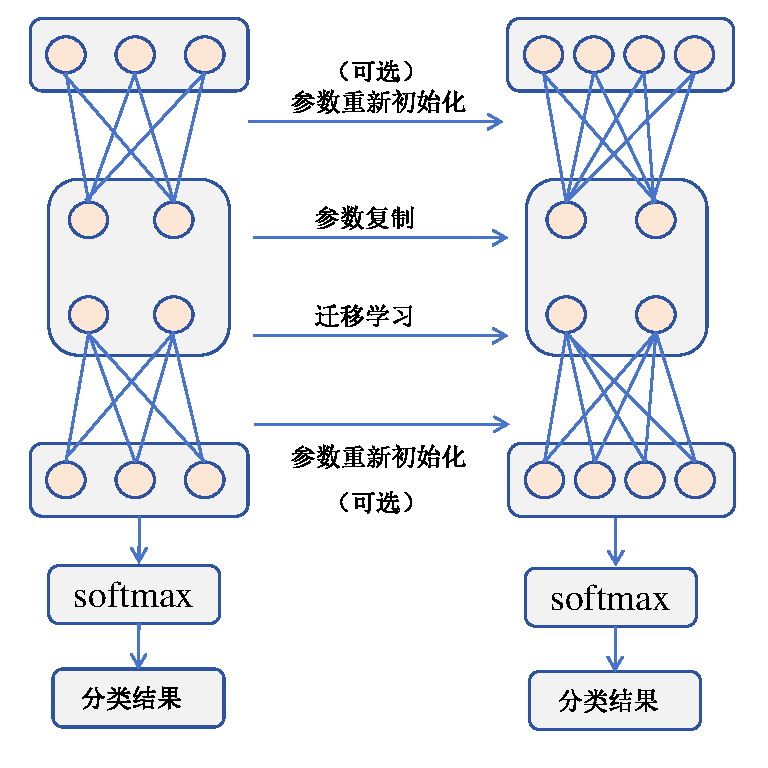
\includegraphics[height=.25\textheight,keepaspectratio]{img/transfer/model_transfer.pdf}
    \caption{模型迁移学习方法}
    \label{fig:model_transfer}
\end{figure}
基于模型微调的迁移学习方法如图\ref{fig:model_transfer}示。当原数据及格式与目标数据集不相同时,需要对模型的结构进行调整。

若输入维度不匹配,通常情况会调整神经网络的第1层,这主要是因为神经网络中靠近输入层的权重往往与数据集中低层次信息有关,当数据集发生变化及低层次语义信息会显著发生变化,原数据集中的权重将不再适用。如果在多分类任务中输出维度不匹配,则会调整神经网络的最后一层,这主要是因为最后一层的输出直接关联具体任务,其维度即为输出的类别数。

本节使用的模型沿用上一章节使用线性编码的模型,当输入的维度发生变化时会丢弃原有的投影矩阵,然后使用新的特征矩阵,实现维度匹配;执行多分类任务时,若样本类别不同则丢弃最后一层全连接层,然后将其进行随机初始化。
\section{基于模型微调的迁移学习}
\begin{figure}
    \centering
    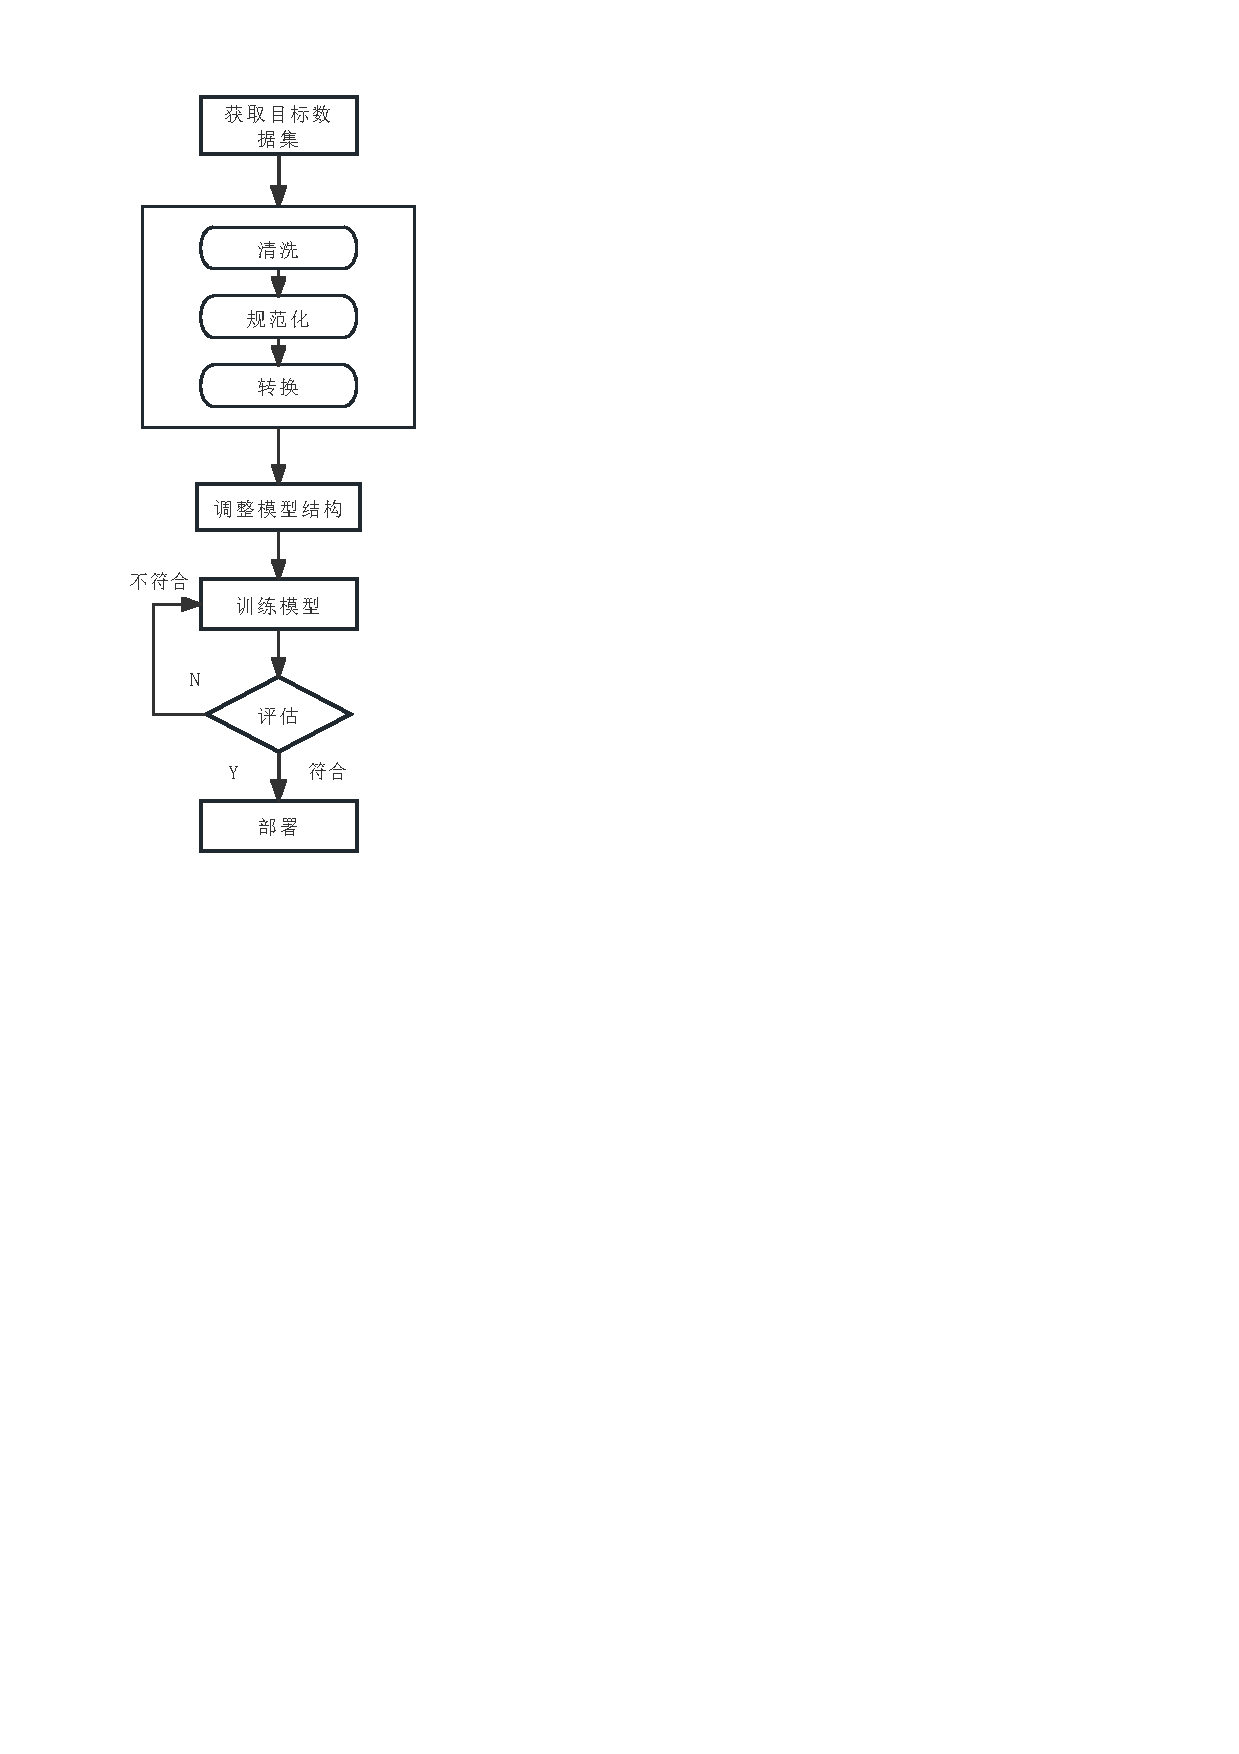
\includegraphics[height=.5\textheight,keepaspectratio]{img/transfer/transfer_method.pdf}
    \caption{迁移学习步骤}
    \label{fig:transfer_method}
\end{figure}
如图\ref{fig:transfer_method}示,将已在原数据集上训练好的模型,迁移到目标数据及步骤如下:
\begin{enumerate}
    \item 目标数据集预处理。预处理对于原始数据集几乎是必做的。在预处理中需要进行数据清洗去除不合理的样本。随后需要将样本中各属性值进行规范化,变换的目的是将数据转化为统一格式,以方便批量处理。最后还需要对样本进行转换,对数值进行转换一般会进行重映射,将数值分布调整到合适范围,以方便模型学习;对于非数值部分可以将其转化为数值,如自然语言处理中,会将单词转换为词向量。
    \item 随后需要将源数据集上训练得到的模型进行转换,以适应目标数据集。
    \item 转换后的模型会在目标数据集上进行训练,每次训练结束后都会进行评估,当模型符合实际需求就可部署到入侵检测系统中,不符合需求就会使用目标数据集进行进一步微调。
\end{enumerate}

\section{基于通用模型的迁移学习}
上述基于模型的信息学习方法最大的缺点已在绪论部分叙述,即没有充分利用数据集提供的信息,以辅助迁移学习过程。另一方面,不同数据集中一些属性的底层特征相同,然而迁移学习为了适应数据集维度的变化,将神经网络中的第1层删除,因此丢失可能对目标数据集有帮助的底层知识。

在前一章节构建了一种对时序建模的通用模型,该模型以数据集中对各属性描述的语义信息作为辅助。当该模型用于迁移学习时,解决了上述两个不足。

首先模型的第1阶段是Transformer编码器,该架构面向变长序列设计,因此具有良好的可扩展性,理论上可以兼容各种格式(不同维度)的输入。在更改数据集时,并不需要对第1层进行重置,对于多分类任务,只需重置最后一层用于分类的权重值。

因此使用通用模型进行迁移学习与使用传统模型进行迁移学习,在过程上有所不同。
\begin{enumerate}
    \item 目标数据集预处理。在使用通用模型进行迁移学习时,预处理仍然是必做的,特别是在第一步需要去除不合理的数据,以及第二步将数据集转化为标准格式,以适应模型的输入。随后需要将样本中各属性值进行重新映射,考虑到其通用性,一些对于数值属性的相对标准化方法可能不再适用。如最大最小值归一化。而使用其他相对标准化方式,如使用对数函数对数值进行变换,所有数值均使用一种函数,保留了各属性之间的相对重要程度。对于文本属性,将其转化为数字索引或独热编码并不合适,而应该使用词向量嵌入,使用前者进行编码,不同数据的同一文本可能会被编成不同形式,而使用后者进行编码,可保证同一文本被编码为同样的向量。
    \item 对于通用模型,数据集格式变化时,只需对模型进行轻微的调整,即在多分类任务中重置最后一层全连接层,二分类任务则不需要进行改动。
    \item 通过上述步骤转换后的模型会继续在目标数据集上进行训练,每次训练除了提供数据以及对应标签外,还需提供对该数据的描述文本信息,每次训练结束后进行评估,符合要求则进入部署阶段。
\end{enumerate}

在实际迁移学习训练过程中不会使用多个数据集,各类别描述在训练过程中为常量值。为节省计算量,可通过在初始化模型时将数据集中各属性的描述信息提前通过语言模型生成描述向量。因此在数据预处理步骤的文本编码过程中,除了对数据中的词建立词表还需对数据集各属性描述建立描述向量表。随后在第二步模型初始化过程中替换原有模型的词表以及描述向量表,即可完成模型迁移过程。

\subsection{迁移学习评估}
将KDDCUP-99数据集按照不同的比例进行划分,用以探究在不同数据量下模型迁移的效果。

如表\ref{tab:transfer-exp-acc}示本章提出的通用模型具有非常强的泛化能力,仅需0.02\%的数据即1024个数据包就可成功识别到所给定数据中的两类,而同样的传统模型,则只能识别到给定数据中数量最多的那一类,且模型过拟合。在数据量超过1\%后,模型的正确率也优于传统模型,仅数据量在1‰ $\sim$ 1\%时传统模型才优于本章提出的模型。
\begin{table}[htbp]
\caption{KDDCUP-99数据集上迁移能力评估实验}
    \centering
    \begin{adjustbox}{max width=\textwidth}
    \begin{tabular}{lllllllllllll}
    \toprule
        ~ & 数据& 使用量& 0.0001 &  0.0002&0.0005& 0.001& 0.002 & 0.005 & 0.01 & 0.02 & 0.05 & 0.1 \\ \midrule
        exp1 & acc & all & 0.7928 &  0.7928 &0.7653 & 0.7927 & 0.9888 & 0.9921 & 0.9921 & 0.9941 & 0.9964 & 0.9971 
\\ 
        exp2 & acc & all & 0.7928 &  0.8167 &0.9658 & 0.9564 & 0.9766 & 0.9957 & 0.9916 & 0.9948 & 0.9978 & 0.9982 \\
    \bottomrule
    \end{tabular}
    \end{adjustbox}
    \label{tab:transfer-exp-acc}
\end{table}

如表\ref{tab:transfer-exp-f1}示在数据量较少时传统模型直接对这些较少的类别判定为不存在(f1值为0),而本章提出的模型则正确识别到了这些类别即准确率大于个数最多的类别(拒绝服务)在模型中的占比。

\begin{table}[htbp]
\caption{KDDCUP-99数据集上迁移能力评估实验}
    \centering
    \begin{adjustbox}{max width=\textwidth}
    \begin{tabular}{lllllllllllll}
    \toprule
        ~ & 数据& 使用量& 0.0001 &  0.0002&0.0005& 0.001& 0.002 & 0.005 & 0.01 & 0.02 & 0.05 & 0.1 \\ \midrule
        exp1 & f1& BENIGN& 0.0000 &  0.2458 &0.9303 & 0.8908 & 0.9426 & 0.9912 & 0.9927 & 0.9914 & 0.9948 & 0.9958 
\\ 
        exp1 & f1& Probe& 0.0000 &  0.0000 &0.3764 & 0.7150 & 0.6904 & 0.7858 & 0.3115 & 0.7680 & 0.9352 & 0.9701 
\\
 exp1 & f1& Denial-of-Service& 0.8844 & 0.8965 & 0.9843 & 0.9744 & 0.9872 & 0.9989 & 0.9962 & 0.9979 & 0.9994 &0.9992 
\\
 exp1 & f1& U2R& 0.0000 & 0.0000 & 0.0000 & 0.0000 & 0.0000 & 0.0000 & 0.0000 & 0.0000 & 0.0202 &0.0000 
\\
 exp1 & f1
& R2L& 0.0000 & 0.0000 & 0.0000 & 0.0000 & 0.0000 & 0.0000 & 0.0010 & 0.0000 & 0.1739 &0.5116 
\\
 exp2 & f1& BENIGN& 0.0000 & 0.0000 & 0.9593 & 0.0000 & 0.9863 & 0.9900 & 0.9918 & 0.9884 & 0.9932 &0.9949 
\\
 exp2 & f1
& Probe& 0.0000 & 0.0000 & 0.0423 & 0.0000 & 0.1828 & 0.3647 & 0.4178 & 0.6531 & 0.8263 &0.9248 
\\
 exp2 & f1
& Denial-of-Service& 0.8844 & 0.8844 & 0.8320 & 0.8844 & 0.9958 & 0.9971 & 0.9965 & 0.9987 & 0.9990 &0.9991 
\\
 exp2 & f1& U2R& 0.0000 & 0.0000 & 0.0000 & 0.0000 & 0.0000 & 0.0000 & 0.0000 & 0.0000 & 0.0000 &0.0000 
\\
 exp2 & f1& R2L& 0.0000 & 0.0000 & 0.0000 & 0.0000 & 0.0000 & 0.0000 & 0.0073 & 0.0000 & 0.0000 &0.1732 
\\
    \bottomrule
    \end{tabular}
    \end{adjustbox}
    \label{tab:transfer-exp-f1}
\end{table}

将迁移后的结果与KDDCUP-99数据集上其他入侵检测方法比较,如表\ref{tab:compare_transfer_other}示,相比传统方式的迁移学习,使用通用模型进行迁移学习可达到更高准确率,多模态通用模型在实际网络安全场景中具有应用潜力。

\begin{table}[htbp]
    \centering
        \caption{KDDCUP-99数据集上与其他方法的对比}
    \begin{tabular}{lll}
    \toprule
        模型 & 数据集使用量 & 准确率 \\ \midrule
        基于通用模型的迁移学习& 0.1&99.82\%\\
        Hierarchical IDS\cite{10.3390/sym12020203} & 0.1 & 99.80\% \\
        基于非通用模型的迁移学习& 0.1&99.71\%\\
        CNID\cite{10.1155/2020/4705982}& 0.1 & 98.02\% \\
        FGLCC-CFA\cite{10.1016/j.jisa.2018.11.007}& 0.1 & 95.03\% \\
        \bottomrule
    \end{tabular}

    \label{tab:compare_transfer_other}
\end{table}

\subsection{可视化分析}


\begin{figure}[htbp] % 创建一个新的figure环境
\centering % 居中对齐所有的子图

\subfloat[训练后激活值分布情况]{ % 插入第一个子图及其标题
\begin{minipage}{.5\textwidth}
\centering % 居中对齐子图
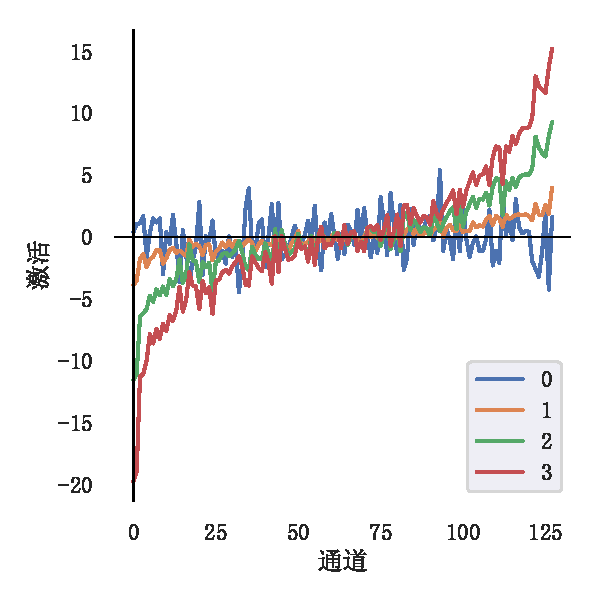
\includegraphics[width=1\linewidth]{img/transfer/activation_t.pdf} % 插入SVG图片
\label{fig:dist_t} % 子图的标签,用于交叉引用
\end{minipage}%
}
\subfloat[初始化时激活值分布情况]{ % 插入第二个子图及其标题
\begin{minipage}{.5\textwidth}
\centering
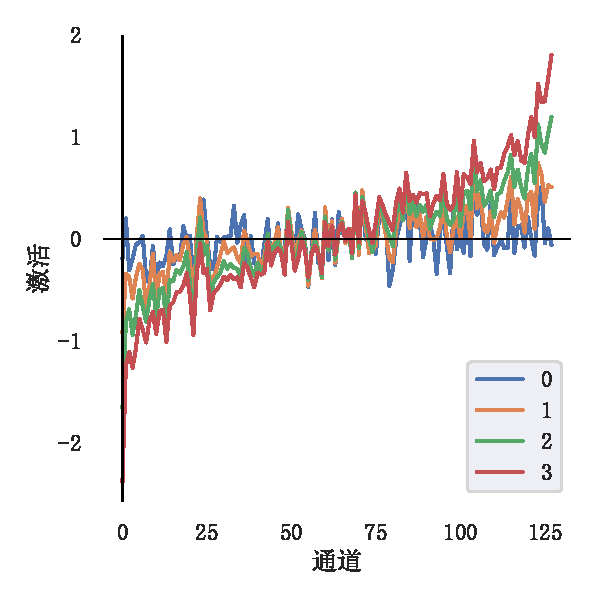
\includegraphics[width=1\linewidth]{img/transfer/activation_o.pdf} % 插入SVG图片
\label{fig:dist_o}
\end{minipage}
}

\subfloat[训练后激活值热图]{ % 插入第三个子图及其标题
\begin{minipage}{.5\textwidth}
\centering
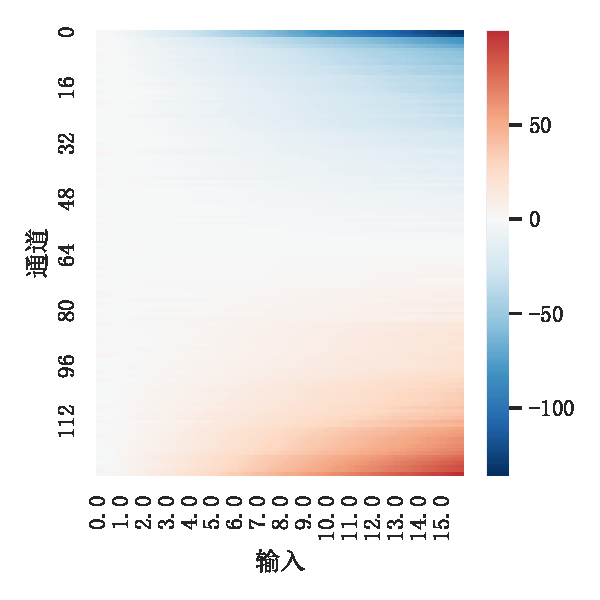
\includegraphics[width=1\linewidth]{img/transfer/channel_act_t.pdf} % 插入PNG图片
\label{fig:hot_t}
\end{minipage}%
}
\subfloat[初始化时激活值热图]{ % 插入第四个子图及其标题
\begin{minipage}{.5\textwidth}
\centering
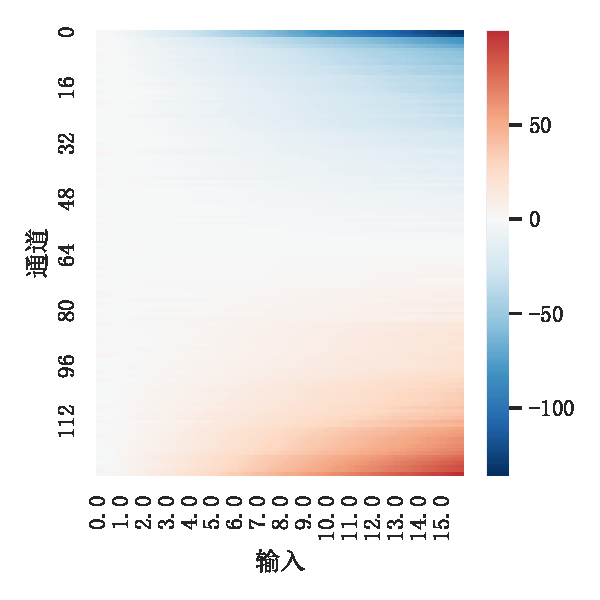
\includegraphics[width=1\linewidth]{img/transfer/channel_act_t.pdf} % 插入PNG图片
\label{fig:hot_o}
\end{minipage}
}

\caption{将数字转化为向量时各通道的激活值(按平均激活值排序)} % 四张图片作为整体的标题
\label{fig:activation_distribution_and_heatmap}
\end{figure}

在网络入侵检测数据集中存在两种数值,一种是分布范围为整个实数域的浮点数,另外一种就是百分比(表示是与否的真假值也可看作特殊百分比)取值范围是[0,1]区间。图\ref{fig:dist_o}与图\ref{fig:dist_t}分别表示初始化与完成训练时该编码器的激活值分布随输入值变化情况。可以看出训练后用于数值映射的多层感知机,成功识别到了这两种数值的不同,对于小于1的数值,多层感知机会将其映射为负的斜率,而将较大的数字往往映射为正的斜率,而且经过训练后,分布更为有序,激活值的绝对值大小扩大了近10倍。


\section{本章小结}

本章主要针对入侵检测模型,在实际部署中可能的困难进行研究。主要利用迁移学习克服因部署环境不同而导致已训练好的模型失效的问题。

对于实际部署环境中数据集格式的差别,常规模型使用基于模型微调的迁移学习方法,同时针对不同格式调整网络结构。对于前一章节提出的通用时序检测模型直接利用数据集中的描述信息提高迁移学习效果,同时由于其通用性,因此不必对网络结构进行调整。

实验结果中发现通用检测模型有较强的泛化能力,在少数据量时能避免模型过拟合,在多数据量时能超越传统迁移学习模型。最后通过与其他方法进行对比证明了基于时序的通用检测模型的有效性。